\documentclass{beamer}
\usepackage{standalone}

\usepackage{stmaryrd}
\usepackage{listings}

\usepackage[hyperref=auto,style=alphabetic]{biblatex}
\addbibresource{kwarc.bib}
\usepackage{appendixnumberbeamer}
\usepackage{tikz}
\usepackage{tikz-qtree}
\usetikzlibrary{arrows.meta}

\usetheme{Pittsburgh}
\setbeamertemplate{footline}[frame number]
\setbeamertemplate{navigation symbols}{}
\usecolortheme{beaver}
\setbeamertemplate{frametitle}[default][left]
\setbeamersize{text margin left=3em}

\usepackage{utils/colors}
\usepackage[forbeamer]{utils/basic}
\usepackage{utils/lstmisc}
\usepackage{utils/lstmmt}

\lstset{basicstyle=\ttfamily}
\lstset{commentstyle=\itshape\color{commentfont}}

\title{GLIF: A Declarative Framework for Symbolic Natural Language Understanding}

\author{\underline{Jan Frederik Schaefer} \and Michael Kohlhase}
\institute{FAU Erlangen-N\"urnberg}
\date{\textbf{FCR 2020} \\ \textit{virtual event due to COVID-19} \\ September 22, 2020 }

\begin{document}
\frame\titlepage

\begin{frame}
    \frametitle{Method of Fragments}
    \only<1-2>{
        \centering
        \only<1>{\def\fraglevel{0}}
        \only<2>{\def\fraglevel{1}}
        \includestandalone{fig/montague-fragments}

        \begin{minipage}[t][2cm]{\textwidth}\vspace{1em}
            How do we get from messy language to formal logic?\\[0.5em]
            \emph{Montague}~\cite{Montague:efl70}: Look at a ``nice'' subset
            and map into logic.
        \end{minipage}
    }

    \only<3>{
        \centering
        \def\fraglevel{1}
        \includestandalone{fig/montague-fragments}
        
        \begin{minipage}[t][2cm]{0.6\textwidth}\vspace{1em}
            \str{Ahmed paints and Berta is quiet.}\\[0.5em]
            \str{Ahmed doesn't paint.}
        \end{minipage}\hfill
        \begin{minipage}[t][2cm]{0.39\textwidth}\vspace{1em}
            $p(a) \wedge q(b)$\\[0.5em]
            $\neg p(a)$
        \end{minipage}
    }

    \only<4>{
        \centering
        \def\fraglevel{2}
        \includestandalone{fig/montague-fragments}
        
        \begin{minipage}[t][2cm]{0.6\textwidth}\vspace{1em}
            \str{Every student paints and is quiet.}\\[0.5em]
            \str{Nobody paints.}
        \end{minipage}\hfill
        \begin{minipage}[t][2cm]{0.39\textwidth}\vspace{1em}
            $\forall x.s(x) \Rightarrow (p(x) \wedge q(x))$\\[0.5em]
            $\neg \exists x.p(x)$
        \end{minipage}
    }

    \only<5>{
        \centering
        \def\fraglevel{3}
        \includestandalone{fig/montague-fragments}

        \begin{minipage}[t][2cm]{0.6\textwidth}\vspace{1em}
            \str{Ahmed isn't allowed to paint.}\\[0.5em]
            \str{Ahmed and Berta must paint.}
        \end{minipage}\hfill
        \begin{minipage}[t][2cm]{0.39\textwidth}\vspace{1em}
            $\neg\lozenge p(a)$\\[0.5em]
            $(\square p(a)) \wedge \square p(b)$
        \end{minipage}
    }
\end{frame}


\begin{frame}
    \frametitle{Method of Fragments}
    If we only hand-wave, we gloss over problems:

    \hspace{2em}\str{Ahmed paints. He is quiet.}
    {$\quad\stackrel{?}{\leadsto}\quad$ \color{logicfont} $p(a)\wedge q(a)$}

    \vspace{1.5em}
    Specify:
    \begin{itemize}
        \item Grammar\com{fixes NL subset}
        \item Target logic
        \item Semantics construction\com{maps parse trees to logic}
    \end{itemize}

    \vspace{1.5em}
    On paper~\cite{Montague:tptoqi73}:\com{difficult to scale}

    \vspace{0.3em}\hspace{2em}
\includegraphics[trim=0 0 0 80,clip,width=0.8\textwidth]{fig/montague-tptoqioe.png}
    % \newcommand\VP{\text{\upshape\tiny VP}}
    % \hspace{2em}$\llbracket\text{\strplain{$P_{\VP}$ and $Q_{\VP}$}}\rrbracket_{\VP} = \lambda x. \llbracket\text{\strplain{$P_{\VP}$}}\rrbracket(x) \wedge \llbracket\text{\strplain{$Q_{\VP}$}}\rrbracket(x)$
\end{frame}

\begin{frame}
    \frametitle{GLIF: Grammatical Logical Inference Framework}
    \centering

    \parbox[t][1em][t]{\textwidth}{
        \centering\textit{
            \only<1-2>{We have a tool for this!}
            \only<3>{It combines existing tools.}
        }
    }

    \vspace{1.5em}
    \only<1-1>{\disablepart{sempragarrow}}
    \only<1-2>{\disablepart{includejupyter}}
    \only<1-2>{\disablepart{gfbox}\disablepart{mmtbox}\disablepart{elpibox}}
    \includestandalone[width=\textwidth]{fig/glif-architecture}

    \vspace{1.5em}
    \begin{minipage}[t][2cm]{\textwidth}
        \only<1-2>{
            \begin{tikzpicture}
                \node(str) at (-4,0) {\str{Ahmed and Berta paint.}};
                % REQUIRES \usepackage{tikz-qtree}
                \node(ast) at (0,0) {\color{nlfont!50!logicfont}
                    \resizebox{1.5cm}{!}{\tikzset{edge from parent/.append style={very thick}}
                    \Tree [ .\textbf{mkS} [ .\textbf{andNP} [ \textbf{Ahmed} \textbf{Berta} ] ] \textbf{paint} ]
                    }};
                \node(log) at (2.8,0) {\color{logicfont}$p(a) \wedge p(b)$};
                \draw[-{Straight Barb[length=6.3,width=5.0]},gray] (str) -- (ast);
                \draw[-{Straight Barb[length=6.3,width=5.0]},gray] (ast) -- (log);
            \end{tikzpicture}
        }
        \only<3>{
            \setlength{\arrayrulewidth}{1.0pt}
            \begin{tabular}{r@{\hskip3pt} l l}
                \vspace{0.1em} &\textbf{GF}   &{(= \textbf{grammar} framework)}\\
                \vspace{0.1em}+&\textbf{MMT}  &{(= \textbf{logic} framework)}\\
                \vspace{0.1em}+&\textbf{ELPI} &{(= \textbf{inference} framework)}\\
                \hline
                \\[-1em]
                =&\textbf{GLIF} &{(= \textbf{natural language understanding} framework)}\\
                \end{tabular}
        }
    \end{minipage}
\end{frame}


\provideenablepart{showspa}
\providedisablepart{showepistemicexample}
\provideenablepart{showjupyter}

\begin{frame}
    \frametitle{Components of GLIF: GF}
    \enablepart{hlgf}
    \includestandalone[width=\textwidth]{fig/glif-architecture}
\end{frame}

\begin{frame}[fragile]
    \frametitle{Components of GLIF: Grammatical Framework \cite{GF:on}}
    \begin{itemize}
        \item Specialized for developing natural language grammars
        \item Separates abstract and concrete syntax\par
            \quad\lstinline[language=GF]|sentence : NP -> VP -> S;               --abstract|\par
            \quad\lstinline[language=GF]|sentence np vp = np.s ++ vp.s!np.n;   --concrete|
        \item Abstract syntax based on LF
        \item Comes with large library \com{$\ge 36$ languages}
    \end{itemize}

    \vspace{2em}
    \hspace{2.5em}\begin{tikzpicture}
        \node(eng) at (-2,0.7) {\str{Ahmed paints}};
        \node(ger) at (-2,-0.7) {\str{Ahmed zeichnet}};
        \node(ast) at (4,0) {
                    \color{logicfont!50!nlfont}
                    \resizebox{2.cm}{!}{\tikzset{edge from parent/.append style={very thick}}
                        \Tree [ .\texttt{sentence} \texttt{ahmed} \texttt{paint} ]
                    }
                };
        \draw[<->, thick] (eng) to node[above,rotate=-9]{Eng. concr. syn.} (ast);
        \draw[<->, thick] (ger) to node[below,rotate=9]{Ger. concr. syn.} (ast);
    \end{tikzpicture}
\end{frame}

\begin{frame}
    \frametitle{Components of GLIF: MMT}
    \enablepart{hlmmt}
    \includestandalone[width=\textwidth]{fig/glif-architecture}
\end{frame}

\begin{frame}[fragile]
    \frametitle{Components of GLIF: MMT}
    \lstset{frame=single}
    \begin{itemize}   
        \item Modular logic development and knowledge representation
        \item Not specialized in one logical framework \com{we use LF}
        \item We will use MMT to:
        \begin{itemize}
            \item { \only<2>{\bf\color{hlfont}} represent abstract syntax }
            \item { \only<3>{\bf\color{hlfont}} specify target logic and discourse domain theory}
            \item { \only<4>{\bf\color{hlfont}} specify semantics construction}
        \end{itemize}
    \end{itemize}
    \lstset{basicstyle=\footnotesize\ttfamily}
    
    \vspace{1em}
    \begin{minipage}[t][4cm]{\textwidth}
        \centering
        \only<2>{% Used in slides/glif-components.tex
% Has to be in separate file...
\begin{minipage}[t]{0.35\textwidth}
    \parbox[t][1em][t]{\textwidth}{\centering\bf GF}\par
    \begin{lstlisting}[language=GF,linewidth=\textwidth]
cat
  NP; VP; S;
fun
  sentence :
    NP -> VP -> S;
    \end{lstlisting}
\end{minipage}
\begin{minipage}[t]{0.1\textwidth}\vskip3em \centering\LARGE$\mapsto$\end{minipage}
\begin{minipage}[t]{0.3\textwidth}
    \parbox[t][1em][t]{\textwidth}{\centering\bf MMT}\par
    \begin{lstlisting}[language=MMT,linewidth=\textwidth]
NP : type
VP : type
S  : type
sentence :
  NP \raa VP \raa S \end{lstlisting}
\end{minipage}
}
        \only<3>{% Used in slides/glif-components.tex
% Has to be in separate file...
\begin{minipage}[t]{0.45\textwidth}
    \parbox[t][1em][t]{\textwidth}{\centering\bf Logic}\par
    \begin{lstlisting}[language=MMT,linewidth=\textwidth]
o : type //propositions
\neg : o \raa o
\wedge : o \raa o \raa o
\vee : o \raa o \raa o

\iota : type //individuals
\forall : (\iota \raa o) \raa o
\exists : (\iota \raa o) \raa o \end{lstlisting}
\end{minipage}\hskip2em
\begin{minipage}[t]{0.3\textwidth}
    \parbox[t][1em][t]{\textwidth}{\centering\bf Domain Theory}\par
    \begin{lstlisting}[language=MMT,linewidth=\textwidth]
paint : \iota \raa o
quiet : \iota \raa o
ahmed : \iota
berta : \iota \end{lstlisting}

    \footnotesize
    \vspace{1.5em}
    \hskip-1em
    idea:
    $\forall f$
    or $\forall \lambda x.f(x)$\par
    \hskip-1em instead of $\forall x.f(x)$
\end{minipage}
}
        \only<4>{\textbf{Semantics Construction}

\ifpart{narrowslides}{\small}{}
\textit{map symbols in abstract syntax to terms in logic/domain theory}

\vspace{0.5em}
\begin{minipage}[t]{0.4\textwidth}
\parbox[t][1em][t]{\textwidth}{\centering Simple setting}\par
\ifpart{switchtomathexample}{
    \lstinputlisting[language=MMT]{slides/misc/snippets/s000.txt}
}{
    \lstinputlisting[language=MMT]{slides/misc/snippets/s001.txt}
}
\end{minipage}
\hspace{1em}
\begin{minipage}[t]{0.5\textwidth}
\parbox[t][1em][t]{\textwidth}{\centering More advanced}\par
\ifpart{switchtomathexample}{
    \lstinputlisting[language=MMT]{slides/misc/snippets/s002.txt}
}{
    \lstinputlisting[language=MMT]{slides/misc/snippets/s003.txt}
}
\end{minipage}
}
    \end{minipage}
\end{frame}

\begin{frame}[fragile]
    \frametitle{Example: Parsing + Semantics Construction}
    {\centering\str{Ahmed and Berta paint}\par}\vspace{1em}
    \hspace{0.49\textwidth}$\downarrow_{\text{parsing}}$\par\vspace{1em}
    {\centering\color{logicfont!50!nlfont} sentence (andNP ahmed berta) paint\par}\vspace{1em}
    \hspace{0.49\textwidth}$\downarrow_{\text{semantics construction}}$\par\vspace{1em}
    {\centering\begin{adjustbox}{}\color{logicfont}\footnotesize\lstinline[language=MMT]|(\lambdan.\lambdav.n v) ((\lambdaa.\lambdab.\lambdap.a p \wedge b p) (\lambdap.p ahmed) (\lambdap.p berta)) paint|\end{adjustbox}\par}\vspace{1em}
    \hspace{0.49\textwidth}$\downarrow_{\text{$\beta$-reduction}}$\par\vspace{1em}
    {\centering\color{logicfont}\small\begin{adjustbox}{}\lstinline[language=MMT]|paint ahmed \wedge paint berta|\end{adjustbox}\par}
\end{frame}

\begin{frame}
    \frametitle{Components of GLIF: ELPI}
    \enablepart{hlelpi}
    \includestandalone[width=\textwidth]{fig/glif-architecture}
\end{frame}

\provideenablepart{mentionprovergen}
\begin{frame}[fragile]
    \frametitle{Components of GLIF: ELPI}
    \begin{itemize}
        \item Implementation and extension of $\lambda$Prolog\com{$\approx$ Prolog + HOAS}
        \item MMT can generate logic signatures
        \ifpart{mentionprovergen}{
            \item First experiments with prover generation
        }{}
        \item Generic inference/reasoning step after semantics construction
        \item Goal: Use it for semantic/pragmatic analysis
    \end{itemize}
    \lstset{basicstyle=\footnotesize\ttfamily}

    \vspace{1em}
    \centering
    % Used in slides/glif-components.tex
% Has to be in separate file...
\begin{minipage}[t]{0.35\textwidth}
    \parbox[t][1em][t]{\textwidth}{\centering\bf MMT}\par
    \begin{lstlisting}[language=MMT,linewidth=\textwidth]
o : type //propositions
\neg : o \raa o
\wedge : o \raa o \raa o
\vee : o \raa o \raa o

\iota : type //individuals
\forall : (\iota \raa o) \raa o
\exists : (\iota \raa o) \raa o \end{lstlisting}
\end{minipage}\hskip2em
\begin{minipage}[t]{0.35\textwidth}
    \parbox[t][1em][t]{\textwidth}{\centering\bf ELPI}\par
    \begin{lstlisting}[language=ELPI,linewidth=\textwidth]
kind o type.
not : o -> o.
and : o -> o -> o.
or  : o -> o -> o.

kind i type.
type forall (i -> o) -> o.
type exists (i -> o) -> o.  \end{lstlisting}
\end{minipage}

    \par
%     \begin{minipage}[t]{\textwidth}
%         \centering
%         \begin{minipage}[t]{0.5\textwidth}
%             \begin{lstlisting}[language=ELPI,frame=single]
% kind o type.
% type not o -> o.
% type and o -> o -> o.
% 
% kind i type.
% type forall (i -> o) -> o.
%             \end{lstlisting}
%         \end{minipage}
%     \end{minipage}
\end{frame}

\ifpart{showepistemicexample}{
    \begin{frame}[fragile]
    \def\mybox#1{\square_{#1}}
    \def\mydia#1{\lozenge_{#1}}
    \def\sfiven{{S5_n}}
    \frametitle{Example: Epistemic Q\&A}
    \centering
    \strplain{\makebox[9.5cm][l]{John knows that Mary or Eve knows that Ping has a dog.}\makebox[1.5em]{\upshape($S_1$)}\\
              \makebox[9.5cm][l]{Mary doesn't know if Ping has a dog.}\makebox[1.5em]{\upshape($S_2$)}\\
              \makebox[9.5cm][l]{Does Eve know if Ping has a dog?}\makebox[1.5em]{\upshape($Q$)}}

    {\color{logicfont}
        \begin{align*}
            S_1 &= \mybox{john}(\mybox{mary} hd(ping)\vee \mybox{eve}hd(ping))\\
            S_2 &= \neg(\mybox{mary}hd(ping) \vee \mybox{mary}\neg hd(ping))\\
            Q &= \mybox{eve}hd(ping) \vee \mybox{eve}\neg hd(ping)
        \end{align*}
    }

    \begin{table}
        \begin{tabular}{l l}
            $S_1, S_2 \vdash_\sfiven Q$\quad      &$\leadsto$\quad yes\\
            $S_1, S_2 \vdash_\sfiven \neg Q$\quad &$\leadsto$\quad no\\
            else &$\leadsto$\quad maybe
        \end{tabular}
    \end{table}
\end{frame}

}{}

\ifpart{showspa}{
    \begin{frame}
        \frametitle{Semantic/Pragmatic Analysis}
        {
            \centering
            \str{The trophy doesn't fit in the brown suitcase because it's too big.}~\cite{levesque2012winograd}\par
            \pause
            \str{The trophy doesn't fit in the brown suitcase because it's too small.}~\cite{levesque2012winograd}\par
            \pause
            \vspace{1.5em}
            \str{The ball has a radius of $2m$.}\par
            \str{The ball has a mass of $2m$.}\par
            \vspace{1.5em}
            \str{We saw her duck.}\par
        }
        \vspace{2em}
        $\leadsto$ semantics construction creates preliminary semantic representation(s)
        that gets refined by the semantic/pragmatic analysis

    \end{frame}
}{}


\ifpart{showjupyter}{
\begin{frame}
    \frametitle{Components of GLIF: Jupyter}
    \enablepart{hljupyter}
    \includestandalone[width=\textwidth]{fig/glif-architecture}
\end{frame}

\begin{frame}
    \frametitle{Components of GLIF: Jupyter}
    \begin{itemize}
        \item Unified, notebook-based interface
        \item Supports implementation and testing
        \item Useful for prototype, demos, teaching, \dots
    \end{itemize}

    \centering
    \vspace{1.5em}
    \fbox{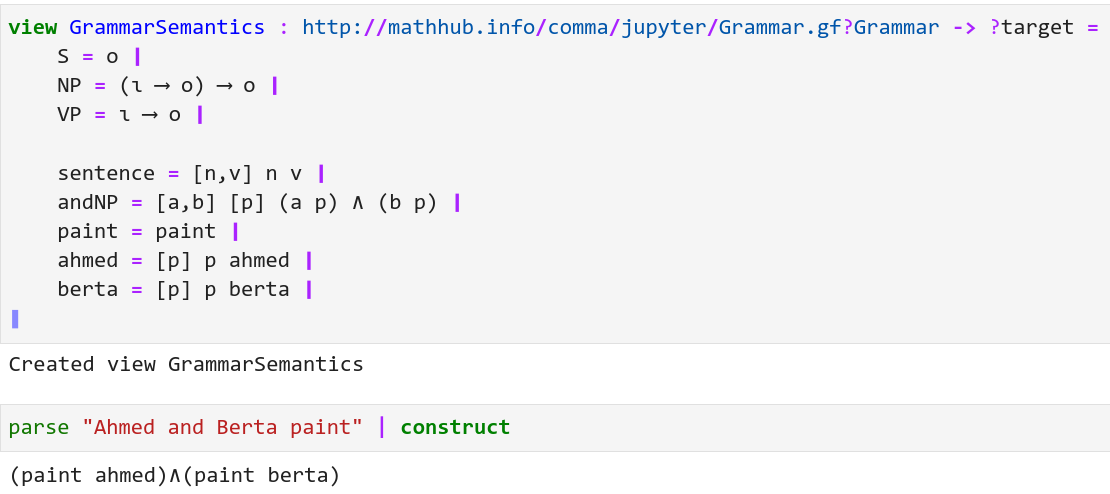
\includegraphics[trim={0 0 20cm 5.7cm},clip,width=0.7\textwidth]{img/screenshot-glif-1.png}}
\end{frame}
}{}


\begin{frame}[allowframebreaks,t]
    \frametitle{References}
    \printbibliography
\end{frame}



\end{document}
